\documentclass[a4paper, 14pt]{extarticle}

\usepackage{../latexDependencies/misc/preamble2}

\geometry{a4paper}

% Название дисциплины
\newcommand{\subject}{Теория вероятности и математическая статистика} 

% Тип работы
% lab - для лабораторной работы 
% hw  - для домашней     работы
\newcommand{\task}{lab} 

% Номер работы
\newcommand{\taskNumber}{5} 

% Название работы
\newcommand{\taskNameOne}{Проверка гипотез о параметрах} 
\newcommand{\taskNameTwo}{нормального распределения.} 

% Имя студента
\newcommand{\studentName}{Очкин Н.В.}

% Имя преподававателя
\newcommand{\teacherName}{Облакова Т.В.}

% Группа
\newcommand{\group}{ФН11-52Б}

% Вариант
\newcommand{\variant}{9}

\begin{document}

\graphicspath{ {../latexDependencies/images} } 
\normalsize

\newcommand{\printTask}{%
    \ifthenelse{\equal{\task}{lab}}{%
        лабораторной%
    }{%
        \ifthenelse{\equal{\task}{hw}}{%
            домашней%
        }{%
            Неизвестный тип задания%
        }%
    }%
}

\begin{titlepage}

    \begin{center}
        {\footnotesize \itshape Федеральное государственное бюджетное 
                       образовательное учреждение высшего образования}
    \end{center}

    \begin{minipage}[c]{0.1\textwidth}
        
\includegraphics[width=1.1\textwidth]{iconBMSTU}
    \end{minipage}
    \hfill
    \begin{minipage}[c]{0.9\textwidth}
        \centering
        \itshape
        \bfseries
        \small
        \guillemotleft Московский государственный технический университет \\
        имени Н.Э. Баумана\guillemotright \\
        (национальный исследовательский университет) \\
        (МГТУ им. Н.Э. Баумана) 
    \end{minipage}

    \vspace{0.5cm}
    \noindent\rule{\textwidth}{2pt} \\

    \noindent\uline{\textbf{ФАКУЛЬТЕТ} ФУНДАМЕНТАЛЬНЫЕ НАУКИ} \\
    \vspace{-5pt} \\
    \noindent\uline{\textbf{КАФЕДРА} ВЫЧИСЛИТЕЛЬНАЯ МАТЕМАТИКА И МАТЕМАТИЧЕСКАЯ} \\
    \vspace{-5pt} \\
    \noindent\uline{ФИЗИКА (ФН11)} \\
    \vspace{-5pt} \\
    \noindent\uline{\textbf{НАПРАВЛЕНИЕ ПОДГОТОВКИ} МАТЕМАТИКА И КОМПЬЮТЕРНЫЕ} \\
    \vspace{-5pt} \\
    \noindent\uline{НАУКИ (02.03.01)} \\

    \begin{center}
        \bfseries
        \textsc{О т ч е т} \\[10pt]
        по \printTask {} работе \textnumero {} \taskNumber
    \end{center}

    \vspace{10pt}

    \hspace{10pt} 
    \noindent \textbf{Название \printTask {} работы:} \par
    \vspace{5pt}
    \hspace{10pt} 
    \noindent \textbf{\uline{\taskNameOne}} \vspace{5pt} \\
    \null\hspace{31pt} 
    \textbf{\uline{\taskNameTwo}} \vspace{5pt} 

    \vspace{10pt}

    \begin{center}
        \bfseries
        Вариант \textnumero {} \variant
    \end{center}

    \vspace{20pt}

    \hspace{10pt} 
    \noindent \textbf{Дисциплина:} \par
    \vspace{10pt}
    \hspace{10pt} 
    \noindent {\large \subject}

    \vspace{10pt}

    \begin{flushright}
        \renewcommand{\arraystretch}{3}
        \begin{tabular}{r r r}
            \multicolumn{1}{l}{Студент группы \uline{\group}} & 
            $\quad \underset{\text{(Подпись, дата)}}{\underline{\hspace{3cm}}} \quad$ & 
            \multicolumn{1}{c}{$\underset{\text{(И.О. Фамилия)}}{\uline{\textbf{\studentName}}}$} \\

            \multicolumn{1}{l}{Преподаватель} & 
            $\quad \underset{\text{(Подпись, дата)}}{\underline{\hspace{3cm}}} \quad$ & 
            \multicolumn{1}{c}{$\underset{\text{(И.О. Фамилия)}}{\uline{\textbf{\teacherName}}}$} \\
        \end{tabular}
    \end{flushright}

    \vfill

    \begin{center}
        \small
        Москва, 2024
    \end{center}
\end{titlepage}


\newgeometry{left=25mm, right=25mm, top=20mm, bottom=20mm}

\graphicspath{ {../latexDependencies/images/LW5} }

% Customize section, subsection, subsubsection and paragraph styles
\titleformat{\section}
  {\normalfont\large\bfseries}{\thesection}{1em}{}

\titleformat{\subsection}
  {\normalfont\normalsize\bfseries}{\thesubsection}{1em}{}

\titleformat{\subsubsection}
  {\normalfont\small\bfseries}{\thesubsubsection}{1em}{}

\titleformat{\paragraph}
  {\small\small\bfseries}{\theparagraph}{1em}{}

\thispagestyle{empty}

\null\newpage

% \setcounter{tocdepth}{5}
% \setcounter{secnumdepth}{5}

% \pagenumbering{roman}

% \tableofcontents
% \newpage

\pagenumbering{arabic}
\setcounter{page}{1}

\setstretch{1}
\linespread{1.1}

\setlength{\parindent}{0pt}

\fontsize{12pt}{16pt}\selectfont

\definecolor{myblue}{HTML}{0A88C2}
\definecolor{myred}{HTML}{FF1B1C}
\definecolor{mygreen}{HTML}{386641}

\lstdefinestyle{mystyle}{
    basicstyle=\ttfamily\footnotesize,
    keywordstyle=\color{myblue},
    stringstyle=\color{myred},
    commentstyle=\color{green!50!black},
    showstringspaces=false,
    frame=leftline, 
    framesep=10pt, 
}

% Set the style for Python code
\lstset{style=mystyle, extendedchars=\true}

% --------------------------------------START--------------------------------------

\section*{Задание}\vspace{-20pt}\rule{\linewidth}{0.1mm}

По данной выборке из нормально распределенной генеральной совокупности:

\begin{enumerate}
    \item постройте критерий $S_2$ уровня $\alpha$ и проверьте гипотезу $H_0: a = a_0$ 
    против односторонней альтернативы $H_2$, если  $\sigma$ неизвестно;
    \item постройте критерий $S_3$ уровня $\alpha$ и проверьте гипотезу $H_{01}: \sigma = \sigma_0$ 
    против альтернативы $H_3$, если $a$ неизвестно;
    \item постройте оптимальный критерий $S_1$ уровня $\alpha$ и проверьте $H_0$ против простой 
    альтернативы $H_1: a = a_1$, если $\sigma = \sigma_1$ известно;
    \item найдите ошибку второго рода $\beta = P(\overline{S_1} | H_1)$ критерий $S_1$;
    \item найдите такие значения $a_1$, для которых ошибка второго рода критерия $S_1$ не 
    превосходит $\varepsilon$;
    \item постройте совмещенные графики гистограммы относительных частот данной выборки и плотностей 
    нормального распределения с параметрами $(a_0, \sigma_1)$ и $(a_1, \sigma_1)$
\end{enumerate}

\section*{Исходные данные}\vspace{-20pt}\rule{\linewidth}{0.1mm}

\vspace{10pt}

\begin{center}
    \begin{tabular}{|c|c|c|c|c|c|c|c|c|c|}
        \hline
        $\alpha$ & $a_0$ & $H_2$ & $\sigma_0$ & $H_3$ & $a_1$ & $H_1$ & $\sigma_1$ & $\varepsilon$ & $n$ \\
        \hline
        0.1 & 3 & $a > a_0$ & 2.1 & $\sigma > \sigma_0$ & 3.5 & $a = a_1$ & 2.2 & 0.1 & 100 \\
        \hline
    \end{tabular}
\end{center}

\begin{equation*}
    \begin{vmatrix}
        -3.442 & 1.295 & 3.672 & 2.354 & 5.238 & 1.136 & 4.421 & 2.071 & 0.269 & 0.894 \\
        8.202 & 0.605 & -2.011 & 3.375 & 3.767 & 1.068 & 2.928 & -0.276 & 4.924 & 3.31 \\
        5.741 & 6.951 & 3.417 & 2.991 & 5.599 & 4.896 & 9.197 & 3.823 & 1.827 & 5.389 \\
        2.504 & 4.212 & -2.021 & 1.891 & 3.689 & 5.366 & 3.117 & 4.641 & 2.968 & 4.645 \\
        3.752 & 4.582 & 3.601 & 0.934 & 2.785 & 3.294 & 4.695 & 1.092 & 3.155 & 4.352 \\
        0.896 & 0.839 & 4.309 & 2.793 & 7.233 & 0.95 & 5.228 & 1.28 & 5.19 & 0.972 \\
        4.562 & 1.915 & 4.243 & 4.495 & 0.648 & 5.34 & 3.294 & 2.791 & 6.805 & 3.474 \\
        3.044 & 5.452 & 2.957 & 7.862 & 4.61 & 1.317 & 5.383 & 3.205 & -1.022 & 3.602 \\
        3.373 & 5.415 & 4.093 & 5.407 & 0.501 & 2.135 & 1.957 & 0.826 & 5.34 & 3.759 \\
        1.735 & -3.277 & 5.101 & 1.43 & 3.494 & 0.545 & 4.699 & 3.44 & 2.85 & 4.33 \\
    \end{vmatrix}
\end{equation*}

\section*{Ход решения работы}
\subsection*{Первоначальная обработка статистических данных}\vspace{-20pt}\rule{\linewidth}{0.1mm}

Обработка статистических данных происходит в среде Jupyter Notebook.

\begin{itemize}
    \item Крайние члены вариационного ряда и размах выборки\\
    Крайние члены вариационного ряда находятся как минимум и максимум выборки:
    \begin{center}
        \begin{lstlisting}[language=Python]
min_ = min(data)
max_ = max(data)

range_ = max_ - min_
        \end{lstlisting}
    \end{center}
    \vspace{-15pt}
    \begin{gather*}
        \text{min}: -3.442 \qquad \text{max}: 9.197 \\
        \omega: 12.639
    \end{gather*}
    \item Группировка данных\\
    Элементы выборки можно объединить в группы и построить интервальный вариационный ряд. 
    Для этого отрезок $\omega$ разбивается на $l$ равных интервалов. Количество интервалов $l$ 
    можно вычислить по правилу Стёрджеса:
    \begin{equation*}
        l = 1 + \lfloor \log_2 N \rfloor,
    \end{equation*}
    где $\lfloor \quad \rfloor$ - обозначение целой части числа.
    \begin{center}
        \begin{lstlisting}[language=Python]
l_ = 1 + int(np.log2(n_))
        \end{lstlisting}
    \end{center}
    \vspace{-15pt}
    \begin{equation*}
        l = 7
    \end{equation*}
    Для группировки данных найдем интервальный шаг:
    \begin{center}
        \begin{lstlisting}[language=Python]
h_ = range_ / l_
        \end{lstlisting}
    \end{center}
    \vspace{-15pt}
    \begin{equation*}
        h = 1.8056
    \end{equation*}
    Найдем границы интервалов, интервалы и середины интервалов группировки:
    \begin{center}
        \begin{lstlisting}[language=Python]
int_boundaries_ = np.array(
    [min_ + i * h_ for i in range(0, l_ + 1, 1)]
)

intervals_ = np.array(
    [(int_boundaries_[i], int_boundaries_[i+1]) for i in range(0, l_, 1)]
)

mid_ranges_ = np.array(
    [sum(interval)/2 for interval in intervals_]
)
        \end{lstlisting}
    \end{center}
    \vspace{-15pt}
    \begin{gather*}
        \text{границы интервалов}: \\
        [-3.442 \quad -1.6364 \quad 0.1691 \quad 1.9747 \quad 3.7803 \quad 5.5859 \quad 7.3914 \quad 9.197] \\[1em]
        \text{интервалы}: \\
        \left[-3.442 \quad -1.6364 \right) \\
        \left[-1.6364 \quad \hphantom{-}0.1691 \right) \\
        \left[\hphantom{-}0.1691 \quad \hphantom{-}1.9747 \right) \\
        \left[\hphantom{-}1.9747 \quad \hphantom{-}3.7803 \right) \\
        \left[\hphantom{-}3.7803 \quad \hphantom{-}5.5859 \right) \\
        \left[\hphantom{-}5.5859 \quad \hphantom{-}7.3914 \right) \\
        \left[\hphantom{-}7.3914 \quad \hphantom{-}9.197 \hphantom{0} \right] \\[1em]
        \text{середины интервалов}: \\ 
        [-2.5392 \quad -0.7336 \quad 1.0719 \quad 2.8775 \quad 4.6831 \quad 6.4886 \quad 8.2942]
    \end{gather*}
    Найдём частоты попадания элементов из выборки в каждый из интервалов:
    \begin{center}
        \begin{lstlisting}[language=Python]
present = lambda el, int_ : int_[0] <= el < int_[1]
freqs_ = np.zeros(l_)
for el in data:
    for j in range(0, l_, 1):
        if present(el, intervals_[j]):
            freqs_[j] += 1 

freqs_[-1] += np.count_nonzero(data == max_)
        \end{lstlisting}
    \end{center}
    \vspace{-15pt}
    \begin{gather*}
        \text{частоты}: \\
        [4. \quad  2. \quad 24. \quad 32. \quad 30.  \quad 5.  \quad 3.]
    \end{gather*}
    Найдем относительные частоты:
    \begin{center}
        \begin{lstlisting}[language=Python]
rel_freqs_ = freqs_ / n_
        \end{lstlisting}
    \end{center}
    \vspace{-15pt}
    \begin{gather*}
        \text{относительные частоты}: \\
        [0.04 \quad 0.02 \quad 0.24 \quad 0.32 \quad 0.3  \quad 0.05 \quad 0.03]
    \end{gather*}
    Проверим, что сумма вероятности равна 1:
    \begin{center}
        \begin{lstlisting}[language=Python]
assert np.sum(rel_freqs_) == 1
        \end{lstlisting}
    \end{center}
    \vspace{-15pt}
    Найдем вектор плотности относительной частоты:
    \begin{center}
        \begin{lstlisting}[language=Python]
rel_freqs_density_ = rel_freqs_ / h_
        \end{lstlisting}
    \end{center}
    \vspace{-15pt}
    \begin{gather*}
        \text{вектор плотности относительной частоты}: \\
        [0.0222 \quad 0.0111 \quad 0.1329 \quad 0.1772 \quad 0.1662 \quad 0.0277 \quad 0.0166]
    \end{gather*}
    Таким образом была произведена группировка статистических данных. 
    Результатом группировки является интервальный вариационный ряд, 
    который можно представить в виде таблицы:\\

    \hspace{-32.5pt}\hrulefill Интервальный вариационный ряд\hrulefill

    \bigskip

    \begin{table}[h!]
        \centering
        \resizebox{0.8\textwidth}{!}{ % Scale the table to the width of the text
        \setlength{\tabcolsep}{10pt} % Add horizontal space between columns
        \begin{tabular}{cccc}
        \toprule
        & & Относительная & \multirow{3}{*}{\makecell{Плотность \\ относительной \\ частоты}} \\
        Интервал & Частота & & \\
        & & Частота & \\
        \midrule
        $\left[-3.442 \quad -1.6364 \right)$ & 4 & 0.04 & 0.0222 \\[1em] 
        $\left[-1.6364 \quad \hphantom{-}0.1691 \right)$ & 2 & 0.02 & 0.0111 \\[1em]
        $\left[\hphantom{-}0.1691 \quad \hphantom{-}1.9747 \right)$ & 24 & 0.24 & 0.1329 \\[1em]
        $\left[\hphantom{-}1.9747 \quad \hphantom{-}3.7803 \right)$ & 32 & 0.32 & 0.1772 \\[1em]
        $\left[\hphantom{-}3.7803 \quad \hphantom{-}5.5859 \right)$ & 30 & 0.30 & 0.1662 \\[1em]
        $\left[\hphantom{-}5.5859 \quad \hphantom{-}7.3914 \right)$ & 5 & 0.05 & 0.0277 \\[1em]
        $\left[\hphantom{-}7.3914 \quad \hphantom{-}9.197 \hphantom{0} \right]$ & 3 & 0.03 & 0.0166 \\
        \bottomrule
        \end{tabular}
        }
    \end{table}

    \item Гистограмма относительных частот
    
    \begin{center}
        \begin{lstlisting}[language=Python]
def buildBar(filename):
    RED = '#6F1D1B'

    _, ax = plt.subplots(figsize=(10, 6))

    x_values = mid_ranges_
    y_values = rel_freqs_density_

    ax.bar(x_values, 
           y_values, 
           width=h_, 
           color='white',
           edgecolor=RED, 
           linestyle='-', 
           linewidth=1.5, 
           align='center')
    
    decorate_plot(ax, int_boundaries_, 'int', '$p^r$', loc=(0, 0))

    plt.savefig(f'{filename}.png', dpi=300, transparent=True)

    plt.show()
        \end{lstlisting}
    \end{center}

    \hspace{-32.5pt}\hrulefill Гистограмма относительных частот \hrulefill

    \begin{center}
        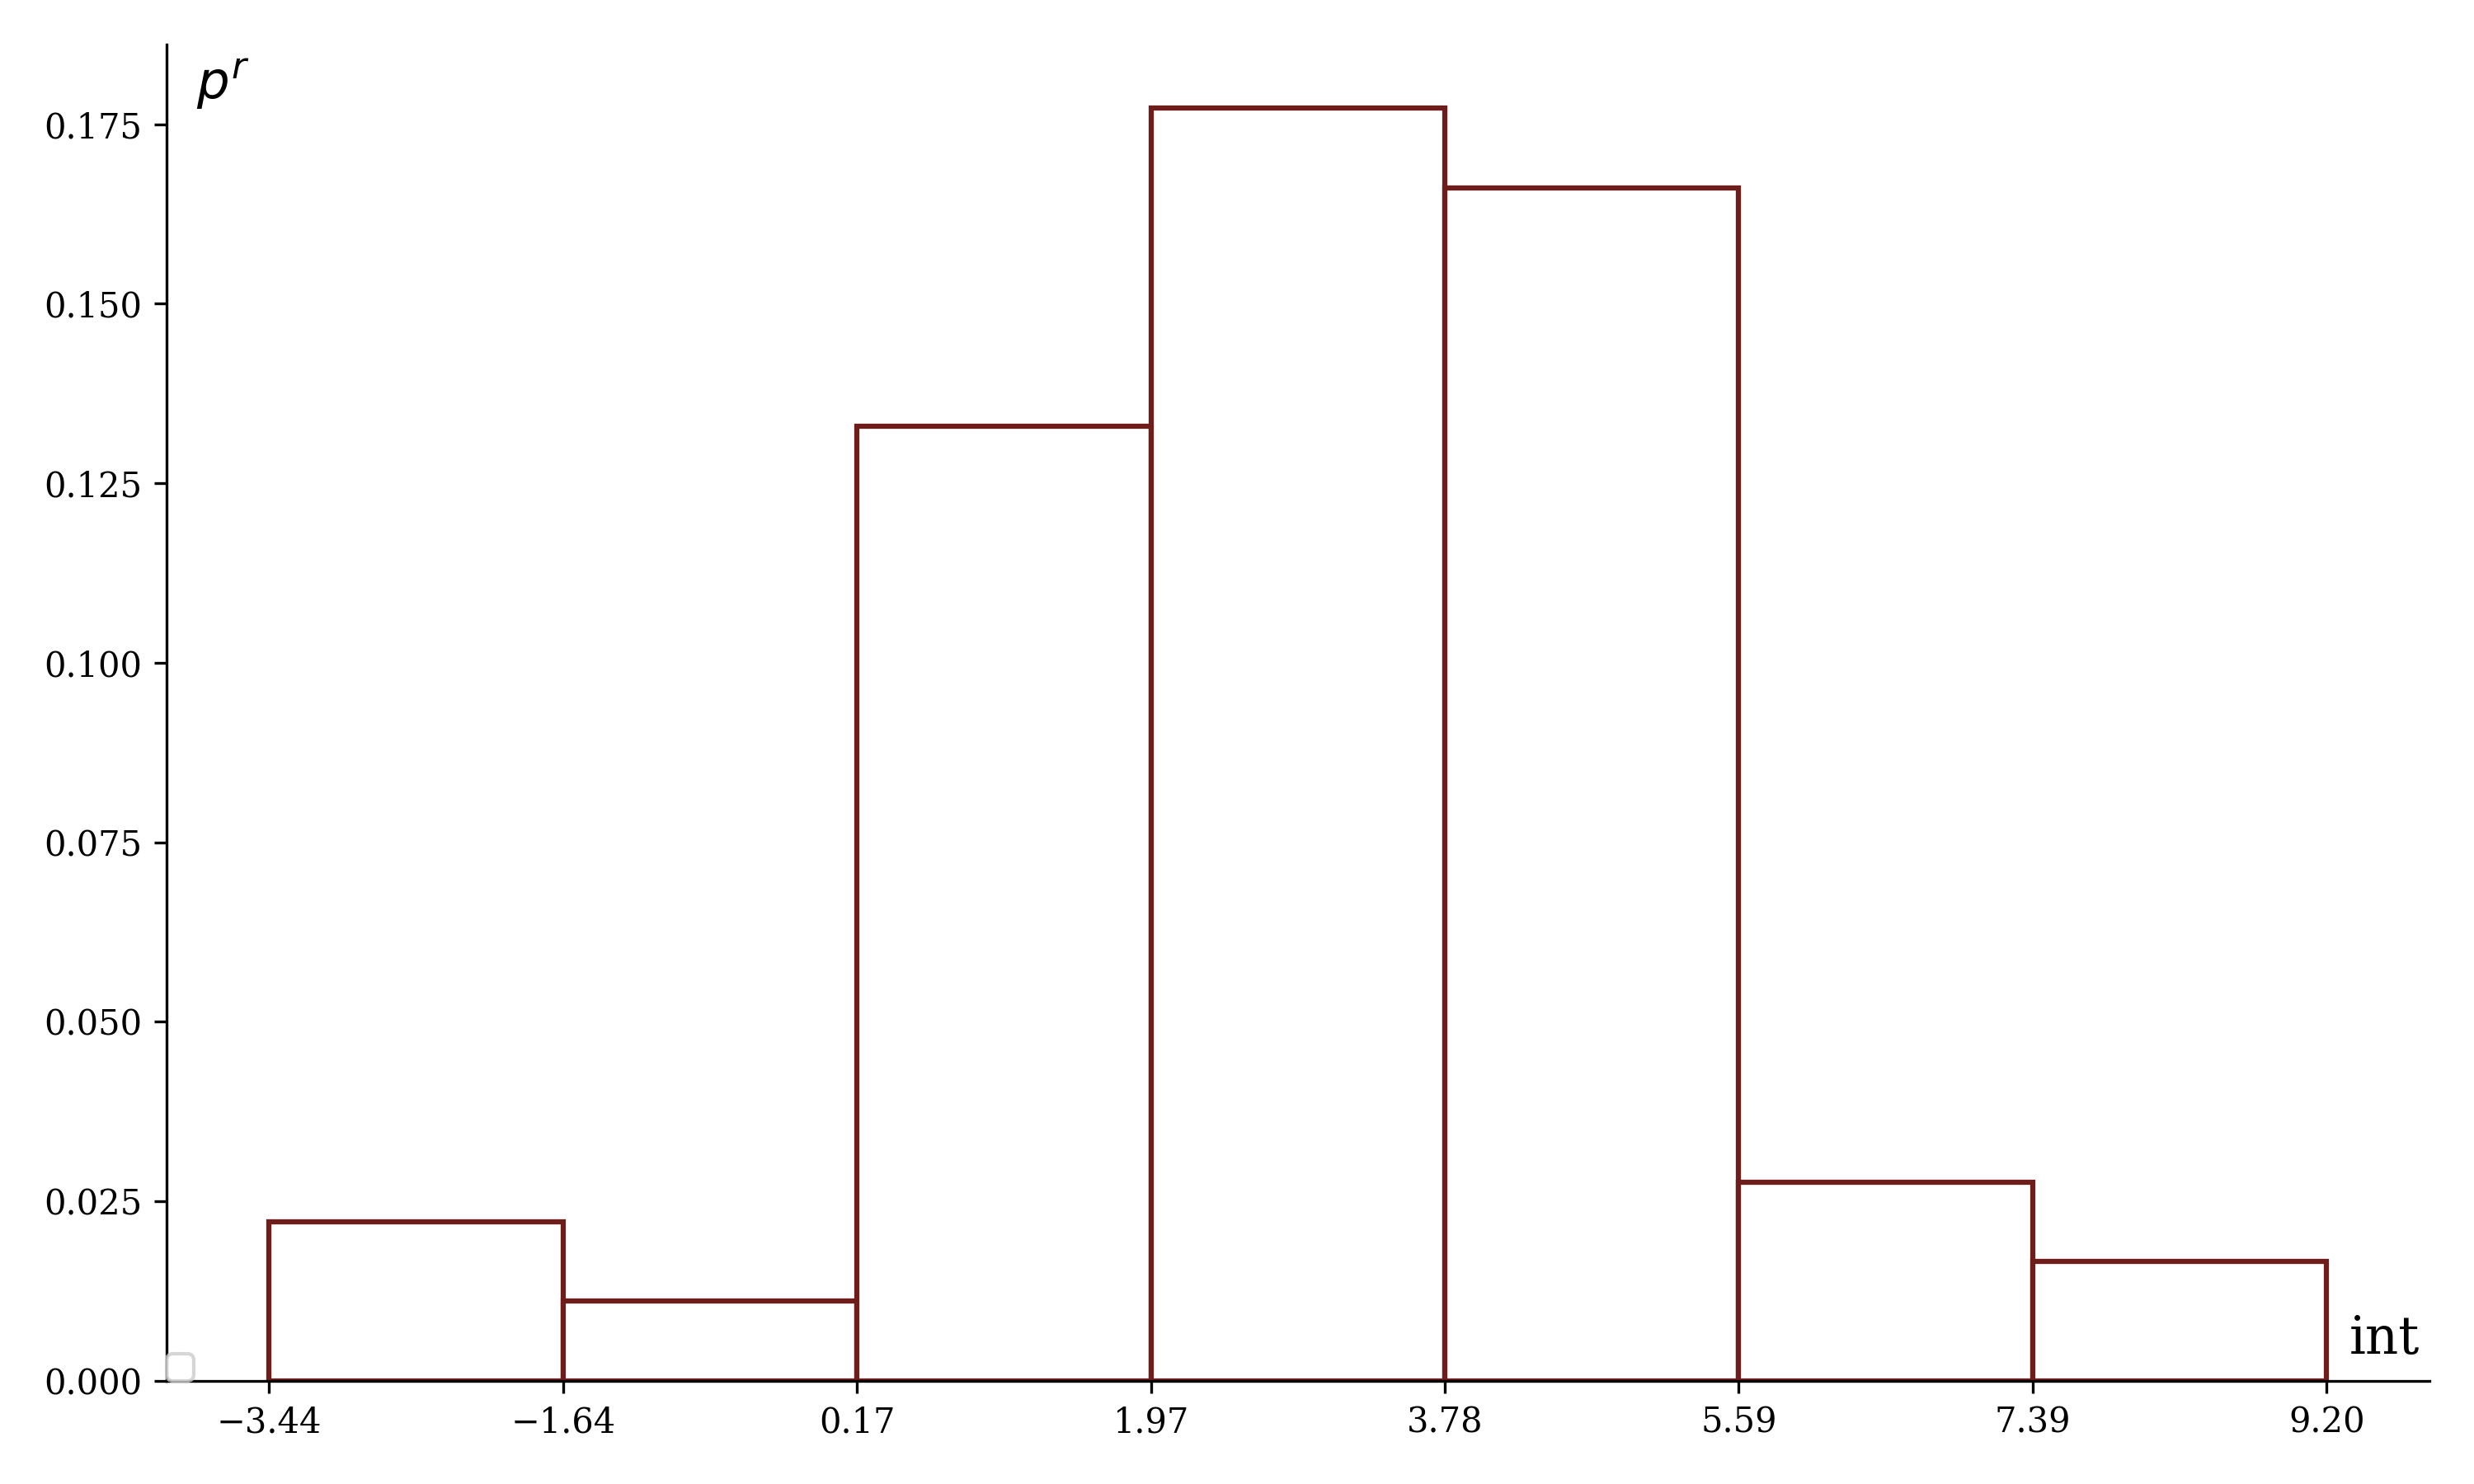
\includegraphics[width=0.8\textwidth]{hist}
    \end{center}

    \item Выборочные характеристики выборки\\
    Найдем выборочное среднее и среднее квадратичное отклонение выборки:
    \begin{center}
        \begin{lstlisting}[language=Python]
overlineX = 1/n_ * sum(data_)

S2 = 1/(n_ - 1) * sum((data_ - overlineX)**2)
        \end{lstlisting}
    \end{center}
    \vspace{-10pt}
    \begin{equation*}
        \overline{X} \approx 3.17705 \qquad S^2 \approx 5.1431775
    \end{equation*}
\end{itemize}

\subsection*{Решение задания}\vspace{-20pt}\rule{\linewidth}{0.1mm}

1. Постройте критерий $S_2$ уровня $\alpha$ и проверьте гипотезу $H_0: a = a_0$ 
против односторонней альтернативы $H_2$, если  $\sigma$ неизвестно.

\begin{equation*}
    \alpha = 0.1 \qquad H_0: a = 3 \qquad H_2: a > 3 \qquad \sigma - \text{неизвестно} \qquad S_2
\end{equation*}

\rule{\linewidth}{0.1mm}

Критическое множество для среднего при альтернативе $H_2: a > 3$ имеет вид:
\begin{equation*}
    S_2 = \left\{ \overline{X} > C_2 \right\}
\end{equation*}

\begin{center}
    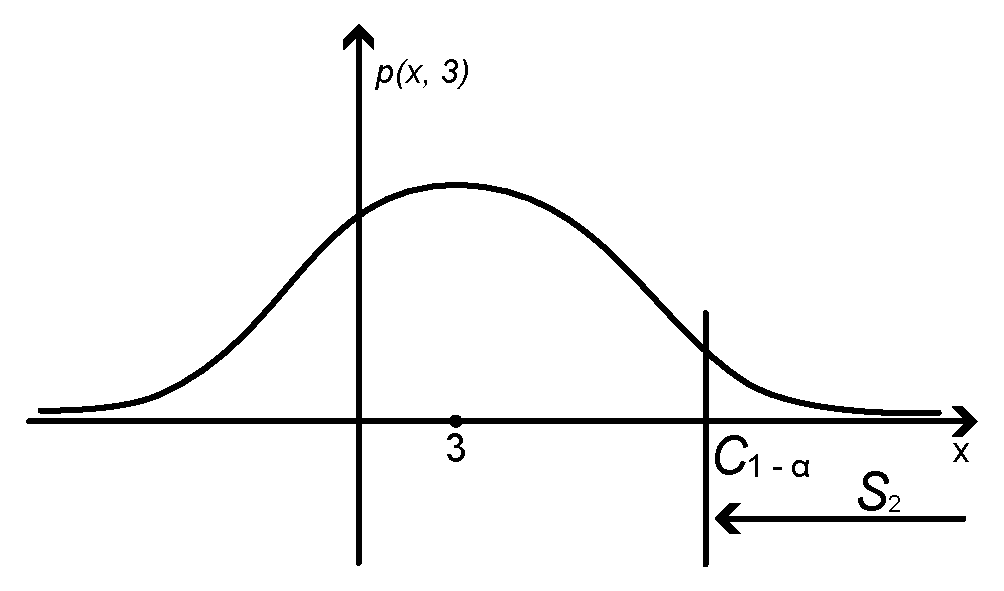
\includegraphics[width=0.6\textwidth]{hypo_plot}
\end{center}

Рассмотрим статистику:

\begin{equation*}
    \cfrac{\overline{X} - a}{S} \sqrt{n} \sim t(n-1)
\end{equation*}

Тогда по определению ошибки первого рода $\alpha = P(S_2 | H_0)$:

\begin{gather*}
    \alpha = P\left(\overline{X} > C_2 | a = 3\right) = 
    P\left(\cfrac{\overline{X} - a_0}{S} \sqrt{n} > 
    \cfrac{C_2 - a_0}{S} \sqrt{n}\right)
    = F_{t(n-1)} \left(\cfrac{C_2 - a_0}{S} \sqrt{n}\right) \\
    \Rightarrow \cfrac{C_2 - a_0}{S} \sqrt{n} = t_{1 - \alpha} (n-1) \\
    \Rightarrow C_2 = \cfrac{S \cdot t_{1-\alpha}(n-1)}{\sqrt{n}} + a_0 \approx 3.29259 
\end{gather*}

\begin{center}
    \begin{lstlisting}[language=Python]
quantile = sp.stats.t.ppf(1-alpha, n_-1)

C2 = np.sqrt(S2)*quantile/np.sqrt(n_) + a0
    \end{lstlisting}
\end{center}

Следовательно, гипотеза $H_0: a = 3$ принимается, потому что $\overline{X} = 3.17705$ 
не принадлежит критическому множеству $S_2 = \left\{ \overline{X} > 3.29259 \right\}$

\rule{\linewidth}{0.1mm}

2. Постройте критерий $S_3$ уровня $\alpha$ и проверьте гипотезу $H_{01}: \sigma = \sigma_0$ 
против альтернативы $H_3$, если $a$ неизвестно.

\begin{equation*}
    \alpha = 0.1 \qquad H_{01}: \sigma = 2.1 \qquad H_3: \sigma > 2.1 \qquad a - \text{неизвестно} \qquad S_3
\end{equation*}

\rule{\linewidth}{0.1mm}

Критическое множество для среднего квадратического отклонения при 
альтернативе $H_3: \sigma > 2.1$ имеет вид:
\begin{equation*}
    S_3 = \left\{ S^2 > C_3 \right\}
\end{equation*}

Рассмотрим статистику:

\begin{equation*}
    \cfrac{S^2 (n-1)}{\sigma^2} \sim \chi^2(n-1)
\end{equation*}

Тогда по определению ошибки первого рода $\alpha = P(S_3 | H_{01})$:

\begin{gather*}
    \alpha = P\left(S^2 > C_3 | \sigma = 2.1\right) = 
    P\left( \cfrac{S^2(n-1)}{\sigma_0^2} > \cfrac{C_3 (n-1)}{\sigma_0^2} \right)
    = \chi^2(n-1) \left(\cfrac{C_3 (n-1)}{\sigma_0^2}\right) \\
    \Rightarrow \cfrac{C_3 (n-1)}{\sigma_0^2} = \chi^2_{1 - \alpha}(n-1) \\
    \Rightarrow C_3 = \cfrac{\chi^2_{1 - \alpha} (n-1)}{n-1} \cdot \sigma_0^2 \approx 5.22994
\end{gather*}

\begin{center}
    \begin{lstlisting}[language=Python]
quantile = sp.stats.chi2.ppf(1-alpha, n_-1)

C3 = quantile * sigma0**2 / (n_ - 1)
    \end{lstlisting}
\end{center}

Следовательно, гипотеза $H_{01}: \sigma = 2.1$ принимается, потому что $S^2 = 5.1431775$ 
не принадлежит критическому множеству $S_3 = \left\{ S^2 > 5.22994 \right\}$

\rule{\linewidth}{0.1mm}

3. Постройте оптимальный критерий $S_1$ уровня $\alpha$ и проверьте $H_0$ против простой 
альтернативы $H_1: a = a_1$, если $\sigma = \sigma_1$ известно.

\begin{equation*}
    \alpha = 0.1 \qquad H_{0}: a = 3 \qquad H_1: a = 3.5 \qquad \sigma = 2.2 \qquad S_1
\end{equation*}

\rule{\linewidth}{0.1mm}

Критическое множество для среднего квадратического отклонения при альтернативе $H_1: a = 3.5$ 
имеет вид:
\begin{equation*}
    S_1 = \left\{ \overline{X} < C_1 \right\}
\end{equation*}

Рассмотрим статистику:
\begin{equation*}
    \cfrac{\overline{X} - a}{\sigma}\sqrt{n} \sim N(0, 1)
\end{equation*}

Тогда по определению ошибки первого рода $\alpha = P(S_1|H_0)$:
\begin{gather*}
    \alpha = P\left(\overline{X} < C_1 | a = 3\right) = 
    P\left( \cfrac{\overline{X} - a_0}{\sigma_1} \sqrt{n} < 
    \cfrac{C_1 - a_0}{\sigma_1} \sqrt{n} \right)
    = \Phi\left(\cfrac{C_1 - a_0}{\sigma_1} \sqrt{n}\right) \\
    \Rightarrow \cfrac{C_1 - a_0}{\sigma_1} \sqrt{n} = u_\alpha \\
    \Rightarrow C_1 = \cfrac{u_\alpha \cdot \sigma_1}{\sqrt{n}} + a_0 \approx 2.7180587 
\end{gather*}

\begin{center}
    \begin{lstlisting}[language=Python]
quantile = sp.stats.norm.ppf(alpha, 0, 1)

C1 = quantile * sigma1 / np.sqrt(n_) + a0
    \end{lstlisting}
\end{center}

Следовательно, гипотеза $H_{0}: a = 3$ принимается, потому что $\overline{X} = 3.17705$ не 
принадлежит критическому множеству $S_1 = \left\{ \overline{X} < 2.7180587 \right\}$

\rule{\linewidth}{0.1mm}

4. Найдите ошибку второго рода $\beta = P(\overline{S_1} | H_1)$ критерий $S_1$.

\rule{\linewidth}{0.1mm}

\begin{gather*}
    S_1 = \left\{ \overline{X} < C_1 \right\} = \left\{ \overline{X} < 2.7180587 \right\} \\
    \cfrac{\overline{X} - a}{\sigma} \sqrt{n} \sim N(0, 1)
\end{gather*}

Согласно определению ошибки второго рода $\beta = P(\overline{S_1}|H_1)$:

\begin{equation*}
    \beta = P(\overline{X} > C_1 | a = 3.5) = P(\cfrac{\overline{X} - a_0}{\sigma_1}\sqrt{n} > 
    \cfrac{C_1 - a_1}{\sigma_1}\sqrt{n}) = 1 - \Phi(\cfrac{C_1 - a_1}{\sigma_1}\sqrt{n}) 
    \approx 0.99981
\end{equation*}

\begin{center}
    \begin{lstlisting}[language=Python]
val = (C1 - a1)/sigma1 * np.sqrt(n_)

beta = 1 - sp.stats.norm.cdf(val, 0, 1)
    \end{lstlisting}
\end{center}

\rule{\linewidth}{0.1mm}

5. Найдите такие значения $a_1$, для которых ошибка второго рода критерия $S_1$ не 
превосходит $\varepsilon$.

\begin{equation*}
    \varepsilon = 0.1
\end{equation*}

\rule{\linewidth}{0.1mm}

\begin{gather*}
    1 - \Phi\left(\cfrac{C_1 - a_1}{\sigma_1} \sqrt{n}\right) <= 0.1 \\
    \Rightarrow \Phi \left( \cfrac{C_1 - a_1}{\sigma_1} \sqrt{n} \right) \leq 0.9 \\
    \cfrac{C_1 - a_1}{\sigma_1} \sqrt{n} = u_{1 - \varepsilon} \\
    \Rightarrow a_1 = \cfrac{-u_{0.9} \cdot \sigma_1}{\sqrt{n}} + C_1 \approx 2.436117
\end{gather*}

\begin{center}
    \begin{lstlisting}[language=Python]
quantile = sp.stats.norm.ppf(1 - epsilon, 0, 1)

a1_ = -quantile * sigma1 / np.sqrt(n_) + C1
    \end{lstlisting}
\end{center}

\rule{\linewidth}{0.1mm}

6. Постройте совмещенные графики гистограммы относительных частот данной выборки и плотностей 
нормального распределения с параметрами $(a_0, \sigma_1)$ и $(a_1, \sigma_1)$.

\rule{\linewidth}{0.1mm}

\begin{center}
    \begin{lstlisting}[language=Python]
def buildBar(filename):
    RED = '#6F1D1B'

    _, ax = plt.subplots(figsize=(10, 6))

    x_values = mid_ranges_
    y_values = rel_freqs_density_

    # hist
    ax.bar(x_values, 
           y_values, 
           width=h_, 
           color='white', 
           edgecolor=RED, 
           linestyle='-', 
           linewidth=1.5, 
           align='center')
    
    x_values = np.linspace(min_, max_, 100)

    # norm pdf with a0 sigma1
    y_values = sp.stats.norm.pdf(x_values, a0, sigma1)
    ax.plot(x_values, 
            y_values, 
            color='black', 
            linestyle='--', 
            linewidth=1.5, 
            label='$N(a_0, \\sigma_1)$')

    # norm pdf with a1 sigma1
    y_values = sp.stats.norm.pdf(x_values, a1, sigma1)
    ax.plot(x_values, 
            y_values, 
            color='blue', 
            linestyle='-', 
            linewidth=1.5, 
            label='$N(a_1, \\sigma_1)$')

    decorate_plot(ax, int_boundaries_, 'int', '$p^r$', loc='best')

    plt.savefig(f'{filename}.png', dpi=300, transparent=True)

    plt.show()
    \end{lstlisting}
\end{center}

\begin{center}
    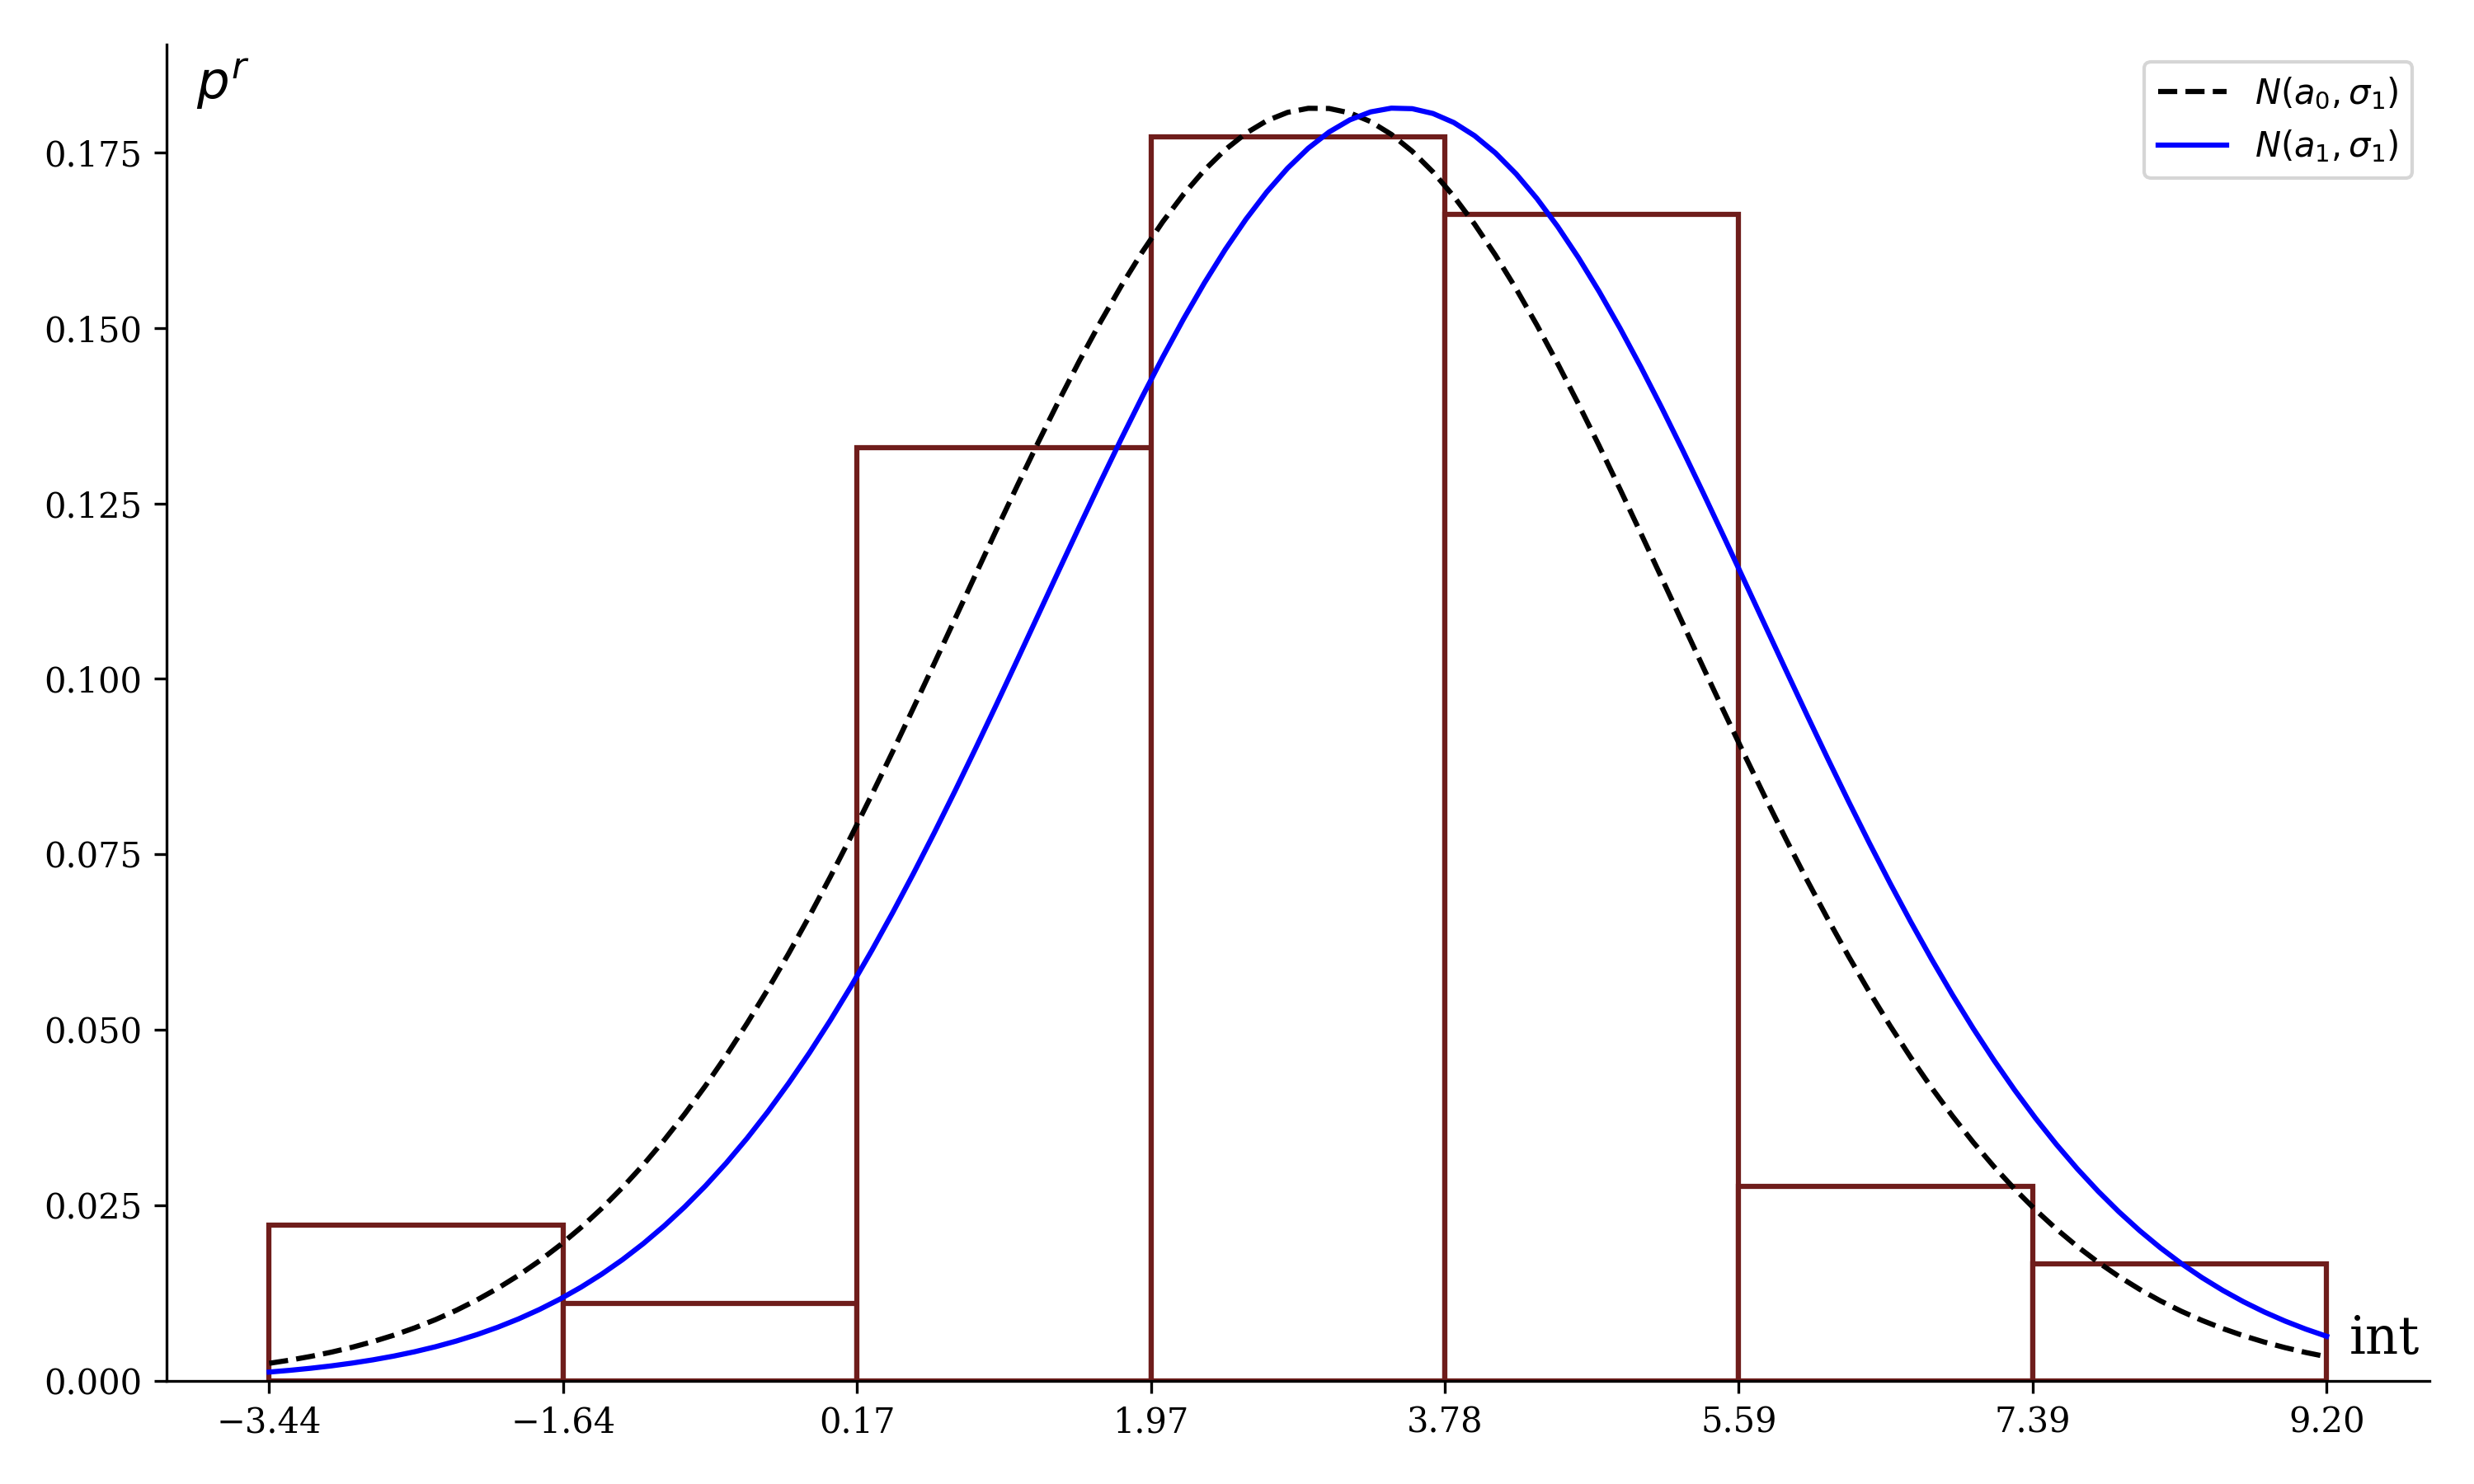
\includegraphics[width=0.9\textwidth]{hist_pdf1_pdf2}
\end{center}

\section*{Вывод}\vspace{-20pt}\rule{\linewidth}{0.1mm}

В процессе выполнения задания мы освоили этапы первоначальной обработки статистических 
данных и изучили основные понятия, связанные с этой темой. Мы научились по заданной выборке 
составлять интервальный вариационный ряд, который является результатом группировки данных, 
а также вычислять выборочное среднее и среднее квадратичное отклонение выборки. 
На следующем этапе был разобран способ построения гистограммы относительных частот. 
Затем, были посчитаны критические множества для среднего и среднего квадратичного отклонения, 
а также проверены 3 гипотезы с разными альтернативами. Была найдена ошибка второго рода для 
критерия $S_1$ и такое значение параметра $a_1$, при котором ошибка второго рода критерия $S_1$ не 
превосходит $\varepsilon$. Также были построены совмещенные графики гистограммы относительных частот $x$ и 
плотностей нормального распределения $N(a_0,\sigma_1 )$ и $N(a_1,\sigma_1 )$. По второму рисунку видно, 
что кривая плотности нормального закона для основной гипотезы $H_0:a=3$ лучше ложится на 
гистограмму, чем в случае альтернативы $H_1:a=3.5$, что согласуется в пункте 3.

% ---------------------------------------CODE---------------------------------------

\newpage

\section*{Приложение}\vspace{-20pt}\rule{\linewidth}{0.1mm}

Программный код, с помощью которого была выполнена данная лабораторная работа.\\

\begin{center}
    \begin{lstlisting}[language=Python]
import numpy as np
import matplotlib.pyplot as plt
import scipy as sp

def decorate_plot(ax, x_ticks, xname, yname, loc=(-0.025, -0.3)):
    SIZE_TICKS = 10

    # Eliminate upper and right axes
    ax.spines['right'].set_color('none')
    ax.spines['top'].set_color('none')

    # Show ticks in the left and lower axes only
    ax.xaxis.set_ticks_position('bottom')
    ax.yaxis.set_ticks_position('left')

    # axis names
    ax.set_xlabel(xname, fontsize=15)
    ax.xaxis.set_label_coords(0.98, 0.05)

    ax.set_ylabel(yname, rotation=0, fontsize=15)
    ax.yaxis.set_label_coords(0.025, 0.95)

    ax.set_xticks(x_ticks)

    # Adjust the font size of the tick labels
    ax.tick_params(axis='both', which='major', labelsize=SIZE_TICKS)

    plt.legend(fontsize=10, loc=loc)

    # Update font settings
    plt.rcParams.update({'font.family': 'serif', 'font.size': 12})

    # Adjust layout
    plt.tight_layout()

data_ = np.array([
    -3.442, 1.295, 3.672, 2.354, 5.238, 1.136, 4.421, 2.071, 0.269, 0.894,
    8.202, 0.605, -2.011, 3.375, 3.767, 1.068, 2.928, -0.276, 4.924, 3.31,
    5.741, 6.951, 3.417, 2.991, 5.599, 4.896, 9.197, 3.823, 1.827, 5.389,
    2.504, 4.212, -2.021, 1.891, 3.689, 5.366, 3.117, 4.641, 2.968, 4.645,
    3.752, 4.582, 3.601, 0.934, 2.785, 3.294, 4.695, 1.092, 3.155, 4.352,
    0.896, 0.839, 4.309, 2.793, 7.233, 0.95, 5.228, 1.28, 5.19, 0.972,
    4.562, 1.915, 4.243, 4.495, 0.648, 5.34, 3.294, 2.791, 6.805, 3.474,
    3.044, 5.452, 2.957, 7.862, 4.61, 1.317, 5.383, 3.205, -1.022, 3.602,
    3.373, 5.415, 4.093, 5.407, 0.501, 2.135, 1.957, 0.826, 5.34, 3.759,
    1.735, -3.277, 5.101, 1.43, 3.494, 0.545, 4.699, 3.44, 2.85, 4.33
])

data_

def group(data):
    n_ = len(data)
    print(f'n: {n_}')

    min_ = min(data)
    max_ = max(data)
    print(f'min: {min_}     max: {max_}')

    range_ = max_ - min_
    print(f'range: {range_}')

    l_ = 1 + int(np.log2(n_))
    print(f'l: {l_}')

    h_ = range_ / l_
    print(f'h: {h_}')

    int_boundaries_ = np.array(
        [min_ + i * h_ for i in range(0, l_ + 1, 1)]
    )
    print(f'interval boundaries: {int_boundaries_}')
    intervals_ = np.array(
        [(int_boundaries_[i], int_boundaries_[i+1]) for i in range(0, l_, 1)]
    )
    print(f'intervals: {intervals_}')
    mid_ranges_ = np.array(
        [sum(interval)/2 for interval in intervals_]
    )
    print(f'intervals\' midpoints: {mid_ranges_}')

    present = lambda el, int_ : int_[0] <= el < int_[1]
    freqs_ = np.zeros(l_)
    for el in data:
        for j in range(0, l_, 1):
            if present(el, intervals_[j]):
                freqs_[j] += 1 

    freqs_[-1] += np.count_nonzero(data == max_)
    print(f'frequencies: {freqs_}')


    rel_freqs_ = freqs_ / n_
    print(f'relative frequencies: {rel_freqs_}')

    assert np.sum(rel_freqs_) == 1

    rel_freqs_density_ = rel_freqs_ / h_
    print(f'relative frequencies\' density: {rel_freqs_density_}')

    print(f'-'*100)

    space_ = ' ' * 5
    for i in range(l_):
        print(f'{intervals_[i]}{space_}{freqs_[i]}{space_}{rel_freqs_[i]}{space_}{rel_freqs_density_[i]}')
    
    return n_, min_, max_, h_, int_boundaries_, mid_ranges_, rel_freqs_density_

n_, min_, max_, h_, int_boundaries_, mid_ranges_, rel_freqs_density_ = group(data_)

def buildBar(filename):
    RED = '#6F1D1B'

    _, ax = plt.subplots(figsize=(10, 6))

    x_values = mid_ranges_
    y_values = rel_freqs_density_

    ax.bar(x_values, 
           y_values, 
           width=h_, 
           color='white',
           edgecolor=RED, 
           linestyle='-', 
           linewidth=1.5, 
           align='center')
    
    decorate_plot(ax, int_boundaries_, 'int', '$p^r$', loc=(0, 0))

    plt.savefig(f'{filename}.png', dpi=300, transparent=True)

    plt.show()

buildBar('hist')

overlineX = 1/n_ * sum(data_)
print(f'mean: {overlineX}')

S2 = 1/(n_ - 1) * sum((data_ - overlineX)**2)
print(f'variance: {S2}')

alpha = 0.1
a0 = 3
sigma0 = 2.1
a1 = 3.5
sigma1 = 2.2
epsilon = 0.1

check = lambda cond : 'accept' if not cond else 'decline'

quantile = sp.stats.t.ppf(1-alpha, n_-1)

C2 = np.sqrt(S2)*quantile/np.sqrt(n_) + a0
print(f'C2 = {C2}, overlineX > C2 = {overlineX > C2} => {check(overlineX > C2)}')

quantile = sp.stats.chi2.ppf(1-alpha, n_-1)

C3 = quantile * sigma0**2 / (n_ - 1)
print(f'C3 = {C3}, S2 > C3 = {S2 > C3} => {check(S2 > C3)}')

quantile = sp.stats.norm.ppf(alpha, 0, 1)

C1 = quantile * sigma1 / np.sqrt(n_) + a0
print(f'C1 = {C1}, overlineX < C1 = {overlineX < C1} => {check(overlineX < C1)}')

val = (C1 - a1)/sigma1 * np.sqrt(n_)

beta = 1 - sp.stats.norm.cdf(val, 0, 1)
print(f'beta = {beta}')

quantile = sp.stats.norm.ppf(1 - epsilon, 0, 1)

a1_ = -quantile * sigma1 / np.sqrt(n_) + C1
print(f'a1\' = {a1_}')

def buildBar(filename):
    RED = '#6F1D1B'

    _, ax = plt.subplots(figsize=(10, 6))

    x_values = mid_ranges_
    y_values = rel_freqs_density_

    # hist
    ax.bar(x_values, 
           y_values, 
           width=h_, 
           color='white', 
           edgecolor=RED, 
           linestyle='-', 
           linewidth=1.5, 
           align='center')
    
    x_values = np.linspace(min_, max_, 100)

    # norm pdf with a0 sigma1
    y_values = sp.stats.norm.pdf(x_values, a0, sigma1)
    ax.plot(x_values, 
            y_values, 
            color='black', 
            linestyle='--', 
            linewidth=1.5, 
            label='$N(a_0, \\sigma_1)$')

    # norm pdf with a1 sigma1
    y_values = sp.stats.norm.pdf(x_values, a1, sigma1)
    ax.plot(x_values, 
            y_values, 
            color='blue', 
            linestyle='-', 
            linewidth=1.5, 
            label='$N(a_1, \\sigma_1)$')

    decorate_plot(ax, int_boundaries_, 'int', '$p^r$', loc='best')

    plt.savefig(f'{filename}.png', dpi=300, transparent=True)

    plt.show()

buildBar('hist_pdf1_pdf2')
    \end{lstlisting}
\end{center}

\end{document}
